\documentclass[12pt]{report}
\usepackage{mathtools}
\usepackage{soul}
\usepackage{titlesec}
\usepackage{graphicx}
\author{Luke Sweeney \\ \large Version 2}
\title{\textbf{Shit I Need to Know} \\ For Calculus 2 \\ UT Arlington}
\date{Spring 2020}

\graphicspath{ {./images/} }

\addtolength{\oddsidemargin}{-0.875in}
\addtolength{\evensidemargin}{-0.875in}
\addtolength{\textwidth}{1.5in}

\addtolength{\topmargin}{-1in}
\addtolength{\textheight}{1.5in}

% \titleformat{\chapter}[display]
%   {\normalfont\bfseries}{}{0pt}{\Large}

\makeindex

\begin{document}
\maketitle
\tableofcontents



Things I need to add:
\begin{enumerate}
	\item Partial fraction decomp
	\item Power series
	\item polar coordinates
	\item parametric equations
	\item volume of rotated curves, shells method
\end{enumerate}


\chapter{Integrals}


\section{$u$-Substitution}
When integrating a function $ f(x) $, if that function contains 1) a sub-function $ u $, and 2) the sub-function's derivative $ du $, then you can perform a $u$-substitution. This is essentially the inverse of the chain rule. It's easier than it sounds. Take the following integral of $ f(x) $

$$ f(x) = 2x \cdot cos(x^2) $$

$$
	\int f(x) \; dx = \int 2x \; cos(x^2) \; dx
$$
There is an inner function $ u = x^2 $ inside $ cos $. This functions derivative $ du = 2x $ also appears in the function. Now we can substitute $u$ into our original integral. The $ 2x $ and $ dx $ are covered by $ du $, and the $ x^2 $ is covered by $ u $. This leaves us with

$$ \int cos(u) \; du = sin(u) = sin(x^2)  $$

\line(1,0){75} \\

Sometimes the coefficients of $u$ will not always match up perfectly. Take the example above, except change the coefficient of $ x^2 $

$$ \int 2x \; cos(4x^2) \; dx $$

Now we must do $ u = 4x^2 $, which means $ du = 8x \; dx $. This doesn't exactly cancel out our $ 2x \; dx $. If we solve $ du = 8x \; dx $ for $ dx $ we get $ dx = \frac{du}{8x} $. We can then substitute $u$ and $dx$ and see what we get

$$ \int 2x \; cos(u) \;  \left( \frac{du}{8x} \right) = \int \frac{1}{4} \; cos(u) \; du $$

$$ = \frac{1}{4} sin(u) = \frac{1}{4} sin(4x^2) $$ 



\line(1,0){75} \\

For definite integrals, there's an extra step. When performing a $u$-substitution, we need to change the bounds of integration \textbf{if} you choose not to back substitute $u$. We'll use the first example above again, but with bounds of integration

$$ \int_0^{\sqrt{\pi}} 2x \; cos(x^2) \; dx $$

We'll do a $u$-substitution and change the bounds. To change the bounds, plug each bound into $ u(x) $:

$$ u(x) = x^2 \quad \quad \quad du = 2x \; dx $$
$$ u(0) = 0^2 = 0 \quad \quad \quad u \left( \sqrt{\pi} \right) = \sqrt{\pi}^2 = \pi $$

$$ \int_0^{\pi} cos(u) \; du = \left[sin(u)\right]_{0}^{\pi} $$

At this point we have two options. We have done a $u$-substitution and changed the bounds of integration. We can evaluate what we found above, \textbf{or} we can use the original bounds and back substitute. Just remember that the old bounds are in terms of $x$ and the new bounds are in terms of $u$. Don't plug in an old bound for $u$ or a new bound for $x$. \\

\begin{itemize}
	\item[] Without back substituting: $ \left[sin(u)\right]_{0}^{\pi} = \left[sin(\pi) - sin(0)\right] = 0 $
	\item[] With back subsituting: $ \left[ sin(x^2) \right]_{0}^{\sqrt{\pi}} = \left[sin(\sqrt{\pi}^2) - sin(0^2) \right] = 0 $
\end{itemize}

Notice the result is the same. It's your choice on which one you want to do. It's easy to skip the step to find the new bounds, which just means to need to back substitute to get the result in terms of $x$.

\clearpage


\section{Integration By Parts}
Given an integral of two products, we should use integration by parts. \\

\textit{Quick note:} Some products can be done with a $u$-substitution, which is simpler than IBP. Try to find a $u$-sub first, and if you can't then try IBP. \\

\noindent The formula for integral by parts is

$$
	\int u \; dv = uv - \int v \; du
$$


There's four elements to IBP: $u$ and $du$, $v$ and $dv$. Why they chose letters that look so similar is lost on me. We're going to assign $u$ and $dv$ to two parts of the integral we are given, then take the derivative of $u$ to get $du$, and take the intergral of $dv$ to get $v$. Once we have all four parts, we can plug them all into the formula. We get to choose what $u$ and $dv$ are (left side of the formula). \\

Lets say we're given the following to integrate

$$ \int xe^x \; dx $$

$$ u = x \quad \quad \quad dv = e^x $$
$$ du = dx \quad \quad \quad v = e^x $$

\noindent I set $u = x$ because it simplifies when taking the derivative, and $dv = e^x \; dx$ because it doesn't get any more complicated when integrating. Choosing which parts to assign to $u$ and $dv$ is the hardest part. After finding $du$ and $v$, we have all the elements we need for the formula

$$ \int x e^x = xe^x - \int e^x \; dx $$
$$ \int x e^x = xe^x - e^x = e^x(x-1) $$

\line(1,0){75} \\

I find the easiest way to remember that the original integral $ = uv - \int v \; du $ is that it's "UV voodoo", because what even is UV? \\

A good way to figure out what to choose for $u$ and $dv$ is through the acronym LIPTE, which stands for "logarithmic", "inverse trig", "polynomial", "trig", and "exponential". There are the type of function you want for $u$, in order. If you have to integrate $ f(x) = xln(x) $, then choose $ u = ln(x) $ becaues "logarithm" comes before "polynomial".

Exponential and trigonometric don't get any simpler when taking the derivative, so assigning them to $u$ doesn't really accomplish anything.  

\clearpage





\section{Trigonometric Substitution}
When given an integral with a sum or difference of squares under a square root, we can use a trig sub. The process for trig subs involves a lot of steps, and they take practice. It's best to just view some examples, which I'll get to in a second. First, here's when to use each trig function and the steps to take for future reference:

\begin{itemize}
	\item[] $ a^2 - x^2 $ \quad \quad $x = asin(\theta)$ \quad \quad $x$ is negative
	\item[] $ x^2 - a^2 $ \quad \quad $x = asec(\theta)$ \quad \quad $x$ is positive
	\item[] $ a^2 + x^2 $ \quad \quad $x = atan(\theta)$ \quad \quad $x$ both are positive
\end{itemize}

\noindent \textbf{Steps:}
\begin{enumerate}
	\item Determine trig function to use and find $x$ in terms of $\theta$ (using table above)
	\item Substitute integral into terms of $\theta$ and simplify using trig identities
	\item Integrate simplified integral (in terms of $\theta$)
	\item Create triangle by solving for $\theta$
	\item Translate result of step 3 into terms of $x$ by reading values off the triangle
	
\end{enumerate}

\line(1,0){75} \\

Let's look at the integral

$$ \int \sqrt{1-x^2} \; dx $$

We can't use $u$-substitution because we would need an $x$ term outside the square root, and we can't use integration by parts because there's no product involved.

(\textbf{Step 1}) It has a difference (or sum) of two squares under a square root, which means we can use a trig substitution. In this case, $ a = 1 $ and the $x^2$ term is negative, so we should use $ x = asin(\theta) $. 

(\textbf{Step 2}) We get $x$ and $dx$ in terms of $\theta$ and substitute. We'll use the trig identity $ sin^2(\theta) + cos^2(\theta) = 1 $ to simplify.

$$ x = sin(\theta) \quad \quad \quad dx = cos(\theta) \; d\theta $$
$$ \int \sqrt{1-x^2} \; dx = \int \sqrt{1-sin^2(\theta)} \; cos(\theta) \; d\theta $$
$$ \sqrt{1-sin^2(\theta)} = \sqrt{cos^2(\theta)} = cos(\theta) $$
$$ \int cos(\theta) cos(\theta) \; d\theta $$
$$ = \int \cos^2(\theta) \; d\theta $$
$$ \int \cos^2(\theta) \; d\theta $$
$$ = \int \frac{1 + cos(2\theta)}{2} $$

(\textbf{Step 3}) We now have a much simpler integral to deal with than the original. We can now integrate to get a result in terms of $\theta$


$$ = \frac{1}{2} \int d\theta + \frac{1}{2} \int cos(2\theta) \; d\theta $$
$$ = \frac{1}{2} \; \theta + \frac{1}{4} sin(2\theta) $$
$$ = \frac{1}{2} \left( \theta +  sin(\theta)cos(\theta) \right) $$

(\textbf{Step 4}) Now we have a result in terms of $\theta$. This is good, but we need to get back in terms of $x$. We're going to do that by creating a triangle.  Remember when we started our trig substitution we had
$$ x = sin(\theta) $$

We're going to solve the first equation for $\theta$ then set up a triangle to help us translate our result back in terms of $x$.

$$ \theta = sin^{-1} \left( \frac{x}{1} \right) $$

You want to make sure you have a fraction inside the inverse trig function, so I put $x$ over 1. Now we have what we need to set up a right triangle. The $sin()$ function is the opposite over the hypotenuse, so we set $ opposite = x $ and $ hypotenuse = 1 $. The remaining side (adjacent) will be the square root we started with ($\sqrt{1-x^2}$). Worship my beautiful triangle: \\

\begin{center}
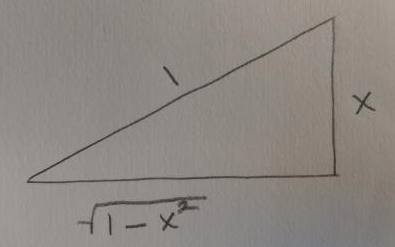
\includegraphics[scale=0.6]{trig_sub_triangle}
$$ \theta = sin^{-1}\left( \frac{x = opposite}{1 = hypotenuse} \right) $$
\end{center}

(\textbf{Step 5}) Now we can just read our values off the triangle we've drawn.

$$ \theta = sin^{-1}(x) \quad \quad \quad sin(\theta) = x \quad \quad \quad cos(\theta) = \sqrt{1-x^2} $$
$$ \frac{1}{2} \left( \theta +  sin(\theta)cos(\theta) \right) $$
$$ = \frac{1}{2} \left( sin^{-1}(x) +  x\sqrt{1-x^2} \right) $$

\clearpage


\section{Improper Integrals}
Some integrals with have bounds of $\infty$, or have a bound that is not defined by the function you're integrating. The solution to this is pretty simple: take the limit of the integral as some number $c\to\infty$. I'm using $c$ because I like it but you can do whatever.

For example, take the integral
$$ \int_1^{\infty} 3x^2 \; dx $$

We have no problems integrating until we get to the evaluation step:
$$ \left[ x^3 \right]_{1}^{\infty} $$

We can't exactly plug in $\infty$ for $x$, so instead we take the limit as $c\to\infty$

$$ \lim_{c\to\infty} \left[ x^3 \right]_{1}^{c} = \lim_{c\to\infty} \left[ (c)^3 - (1)^3 \right] $$

Now it's just a limit problem. In this case, the integral diverges to $\infty$.

\line(1,0){75}

For another example, take this integral
$$ \int_0^1 \frac{1}{x} \; dx = \left[ \ln(x) \right]_0^1 $$

We can't evaluate $\ln(0)$ because it diverges towards $-\infty$. So instead, we take the limit
$$ \lim_{c\to0^+} \left[ \ln(x) \right]_c^1 = \lim_{c\to0^+} \left[ \ln(1) - \ln(c) \right] $$

This integral also diverges, because $\lim_{c\to0^+} \ln(c) \to -\infty$


\clearpage





\chapter{Length, Area, and Volume}

\section{Arc Length of a Curve}
Given a function $f(x)$, the arc length of a segment of the curve from $a$ to $b$ is given by

$$ \int_a^b \sqrt{1+f'(x)^2} $$

\subsection*{Example}
\begin{enumerate}
	\item Find the arc length of $f(x) = \frac{1}{2\sqrt{x}}$ on the interval $[0,4]$ \\
	
	First we find the derivative $f'(x) = \sqrt{x}$, then plug in our values into the formula
	$$ \int_0^4 \sqrt{1+x} \; dx = \int_0^4 \sqrt{u} \; du = \left[ \frac{2}{3} x^{3/2} \right]_0^4 = \frac{2}{3} \left[ (4)^{3/2} - (0)^{3/2} \right] = \frac{16}{3} $$
\end{enumerate}


\section{Surface Area of a Rotated Curve}

Given a function $f(x)$, you can calculate the surface area of the solid made by rotating the curve around the x-axis. The surface area on the interval $[a,b]$ is given by

$$ 2\pi \int_a^b f(x) \sqrt{1+f'(x)^2} \; dx $$

%A visual helps with this
%
%\begin{center}
%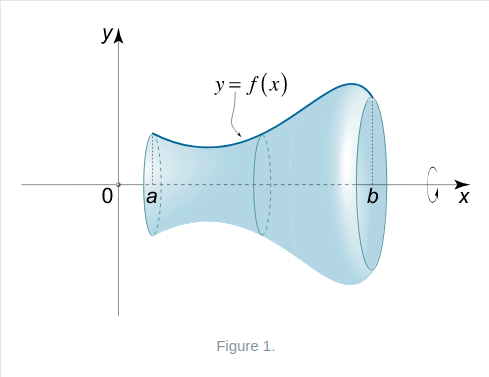
\includegraphics[scale=0.5]{rotated_surface_area}
%\end{center}


\subsection*{Example}

\begin{enumerate}
	\item Find the surface area of the solid generated by rotating $f(x) = \sqrt{4-x^2} $ around the x-axis on the interval $[-1,1]$ \\
	
	First, we find the derivative $ f'(x) = \frac{-x}{\sqrt{4-x^2}} $. 
	
	With the derivative and the bounds, we can plug everything into our formula and evaluate the integral
	
	$$ 2\pi \int_a^b f(x) \sqrt{1+f'(x)^2} \; dx $$
	$$ 2\pi \int_{-1}^{1} \sqrt{4-x^2} \sqrt{1 + \left( \frac{-x}{\sqrt{4-x^2}} \right)^2 } \; dx $$
	$$ = 2\pi \int_{-1}^{1} \sqrt{4-x^2} \sqrt{1 + \frac{x^2}{4-x^2} } \; dx = 2\pi \int_{-1}^{1} \sqrt{4-x^2} \sqrt{\frac{4}{4-x^2} } \; dx $$
	$$ 2\pi \int_{-1}^{1} \sqrt{4-x^2} \frac{2}{\sqrt{4-x^2}} \; dx = 2\pi \int_{-1}^{1} 2 \; dx $$
	$$ 2\pi \left[ 2x \right]_{-1}^{1} = 8\pi $$
\end{enumerate}



\section{Volume of a Rotated Solid}
When a curve is rotated around an axis like in the surface area example above, it creates a solid that has volume.

\subsection{Disk Method}
One way to find this volume is through the \textbf{disk method}. A cross section of any $x$ value on the solid will be a circle, as it's radius (function value at that point) is the same around the entire solid. We can use the equation for the area of a circle $A = \pi r^2$ to help us find the volume. The radius at any $x$ value will be the function value $f(x)$

$$ r = f(x) \quad \text{and} \quad V = \int_a^b \pi r^2 \; dx $$
$$ V = \pi \int_a^b (f(x))^2 \; dx $$

\subsection{Washer Method}
If you need to find the volume of a solid that is defined as the area between two curves rotated around an axis, you can use the \textbf{washer method}. The cross section will be a "washer", or a large circle with a smaller circle removed from the center. Here's an example of a graph that could produce one of these, rotated around the axis. The vertical line represents a typical cross section of the graph

\begin{center}
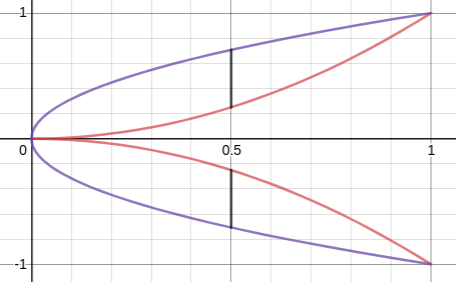
\includegraphics[scale=0.4]{washer_method}
\end{center}


The formula for these is similar to the disk method, but we must subtract the area of the smaller disk. If the upper function is $f(x)$ and the lower function is $g(x)$

$$ V = \left[ \pi \int_a^b f(x)^2 \; dx \right] - \left[ \pi \int_a^b g(x)^2 \; dx \right] $$
$$ V = \pi \int_a^b \left[ f(x)^2 - g(x)^2 \right] dx $$

To find the bounds of integration, find the points here the functions intersect, $f(x) = g(x)$


\subsection*{About The y-axis}
If you need to find the volume or the surface area of a curve rotated around the x-axis, make sure you have a function in terms of $y$. If you're given a function $f(x)$, you need to solve for $y$ and find $f(y)$ and integrate the same way in terms of $y$.

For example, if you're given $f(x) = y = \sqrt{x} $, solve for $x$: $x = f(y) = y^2$ then integrate in terms of $y$.



\clearpage





\chapter{Series}
Here's some basic definitions and random things you should know. I might also put a short reference page in here so you don't have to go looking for stuff. I'll do that later though. 

\section{What are Sequences and Series?}

\begin{itemize}
	\item[] A \textbf{sequence} is a set of numbers, usually denoted by $a_n$ or $a_k$. $n$ or $k$ is the set of all positive integers.
		$$ a_n = n \quad \quad \quad a_n = \left\{ 1, 2, 3, 4, 5, ... \right\} $$
		$$ b_n = \frac{1}{n} \quad \quad \quad b_n = \left\{ 1, \frac{1}{2}, \frac{1}{3}, \frac{1}{4}, ... \right\} $$
		
		
	
	\item[] A \textbf{partial sum} is the sum of a finite number of the terms of a sequence, denoted by $S_n$
		$$ a_n = n \quad \quad \quad S_n = \left\{1 + 2 + 3 + 4 + ... + n\right\} $$
		$$ \quad \quad \; S_3 = \left\{ 1 + 2 + 3 \right\} = 6 $$
		
		
	\item[] A \textbf{series} is the partial sum of a sequence as $n\to\infty$; that is, all the (infinitely many) terms of a sequence added together. It is denoted by the Greek letter sigma ($\Sigma$).
		$$ a_n = n $$
		$$ \sum_{n=1}^{\infty} a_n = \sum_{n=1}^{\infty} n = \left\{ 1 + 2 + 3 + 4 + ... \right\}$$
\end{itemize}

\clearpage

\section{Series Behavior}
When calculating the value of a series (the sum of all the terms of a sequence), the series can behave in a few different ways. If the value of the series continues to increase without bound for each term that we add on, the series \textbf{diverges}.

If the terms of the series grow smaller and smaller and eventually approach 0, the series can level off at an upper bound. In this case, the series \textbf{converges}.

As an example, take the series $ \sum_{n=1}^{\infty} n $. This series is simply the sum of all the positive integers ($1 + 2 + 3...$ to $\infty$). It is easy to imagine that as we add each integer, it grows without bound. Eventually we are adding huge numbers to even bigger numbers. This series diverges.

On the other hand, look at the series $ \sum_{n=1}^{\infty} \left( \frac{1}{n^2} \right) $. Writing out a few of the terms of the series, we get $ 1 + \frac{1}{4} + \frac{1}{9} + \frac{1}{16} ...$ to $ \infty $. While we are adding an infinite number of terms, each one grows smaller and smaller fast enough that the series converges. No matter how many terms we add, it will never grow above a certain value. In this case, this is called a $p$-series, and this particular $p$-series converges to 2; that is, no matter how many terms we add together, the sum will never be greater than 2.

The behavior of some series can be hard to guess. For example, a similar series to the one above is $ \sum_{n=1}^{\infty} \frac{1}{n} $. This particular series is called the "harmonic series". Writing out the first few terms, we get $ 1 + \frac{1}{2} + \frac{1}{3} + \frac{1}{4} ... $ on to infinity. It is true that each term gets smaller, and eventually the terms are going to be very very small. But, in this case, the series still diverges. The amount of terms being added just barely overpowers how small the terms are getting. This series grows \textit{very} slowly, but still diverges. To give you an idea of how slow this series grows, the first 100 terms give a sum of $ \approx 5 $, while adding the first 1,000,000,000 terms gives a sum of $ \approx 21 $. But it is still divergent.


\clearpage




\section{P-Series}
A $p$-series is given by
	$$\sum_{n=1}^{\infty} \left( \frac{1}{n} \right)^p$$
where $p > 0$ by definition. \\


\noindent There is no $p$-series test, but it is a fact of $p$-series that
\begin{enumerate}
	\item If $p > 1$, then the series converges.
	\item If $p \leq 1$, then the series diverges.
\end{enumerate}

\subsection*{Examples}
\begin{enumerate}
	\item Determine if $\sum_{n=1}^{\infty} \frac{1}{n}$ converges or diverges. \\
	
	\textbf{Solution:} This is a common $p$-series called the "harmonic series" with $p = 1$. Because $p = 1$, by part 2 of the $p$-series test this series diverges.
	
	\item Determine if $\sum_{n=1}^{\infty} \left( \frac{3}{n} \right)^2$ converges or diverges. \\
	
	\textbf{Solution:} The $3^2$ can be factored out, and the series can be rewritten as $9 \cdot \sum_{n=1}^{\infty} \left( \frac{1}{n} \right)^2$ where $p = 2$. Because $p > 1$, this series converges by part 1 of the $p$-series test.
	
	\item Determine if $\sum_{n=1}^{\infty} \frac{1}{\sqrt[5]{n}}$ is convergent or divergent. \\
	
	\textbf{Solution:} This is a $p$-series with $p = \frac{1}{5}$, so by part 2 of the $p$-series test it diverges.
\end{enumerate}


\clearpage


\section{Telescoping Series}
There is no set definition of a telescoping series, but this is a type of series where nearly every term is cancelled by another. The sum of the series if the limit of the $nth$ partial sum. 

In almost every case, the easiest way to find the $nth$ partial sum (and by extension, the sum of the series) is to write out a few terms. Let's take the following series and write out the first few terms, then the $n-1$ and $nth$ term. 

    $$ \sum_{k=1}^{\infty} \left( \frac{1}{k} - \frac{1}{k+1} \right) $$

    $$
        S_n = \left( \frac{1}{1} - \frac{1}{2} \right) + \left( \frac{1}{2} - \frac{1}{3} \right) +  \left( \frac{1}{3} - \frac{1}{4} \right) +  \left( \frac{1}{4} - \frac{1}{5} \right) + ...
    $$
    $$
        +  \left( \frac{1}{n-1} - \frac{1}{n} \right) +  \left( \frac{1}{n} - \frac{1}{n+1} \right)
    $$

Looking at the terms in this partial sum, many of the terms cancel out. Cancelling terms and looking at what's left gives us the $nth$ partial sum. We can then take the limit to find the value that the series sums to:

    $$ S_n = 1 - \frac{1}{n+1} $$
    $$ \lim_{n\to\infty} S_n = \lim_{n\to\infty} 1 - \frac{1}{n+1} = 1 $$

\noindent\rule{2cm}{0.4pt}


Some series may not look like telescoping series. You may need to perform a partial fraction decomposition on a problem, or rearrange it in another way which will reveal a telescoping series.

\subsection*{Examples}

\begin{enumerate}
	\item Find the value that the series $ \sum_{k=0}^{\infty} \frac{1}{k^2 + 5k + 6} $ converges to, if it converges. \\
	
	First we need to rearrange this into the form shown above. Ideally, we want the difference of two terms. Let's do a partial fraction decomposition to get
	$$
		\frac{1}{k^2 + 5k + 6} = \left( \frac{1}{k+2} - \frac{1}{k+3} \right)
	$$
	
	Now we can find the $n$th partial sum and take the limit, finding the value the series converges to. We do this by writing out a few terms, then the $n-1$ and $n$th term
	
	$$
		S_n = \left( \frac{1}{2} - \frac{1}{3} \right) + \left( \frac{1}{3} - \frac{1}{4} \right) + \left( \frac{1}{4} - \frac{1}{5} \right) +  \cdots + \left( \frac{1}{n+1} - \frac{1}{n+2} \right) + \left( \frac{1}{n+2} - \frac{1}{n+3} \right)
	$$
	
	You can see that the last term is our original partial fraction. Most of these terms will cancel out. The $-\frac{1}{3}$ will cancel out with the $+\frac{1}{3}$ right next to it, and the same with the $\frac{1}{4}$ and $\frac{1}{5}$ terms. Every term will cancel out except the first $\frac{1}{2}$ and the last $\frac{1}{n+3}$. This leaves us with our partial sum $S_n$. We can take the $lim_{n\to\infty} S_n$ to find the convergence value.
	$$ S_n = \frac{1}{2} - \frac{1}{n+3} $$
	$$ \lim_{n\to\infty} \frac{1}{2} - \frac{1}{n+3} = \frac{1}{2} $$
	
\end{enumerate}




\clearpage


\section{Geometric Series}
Geometric series are series of the form 

    $$ \sum_{n=0}^{\infty} kr^n $$

where $k$ is a constant. For geometric series, the ratio $r$ between any two consecutive terms is a constant; that is, $ \frac{a_{n+1}}{a_n} $ is the same for any value of $n$.

The ratio $r$ can tell you what the series converges to, or if it diverges.
\begin{enumerate}
    \item If $|r| \geq 1$, the series \textbf{diverges}
    \item If $|r| < 1$, the series \textbf{converges} to $\frac{a_1}{1-r}$
\end{enumerate}
See Section \ref{geometric_series_test}: Geometric Series Test on page \pageref{geometric_series_test} for more information and examples.




\clearpage











\chapter{Series Tests}
These are tests to determine the end behavior of a series. Provided here is a list of tests, each with a description and some examples. Tests are not listed in any particular order other than what I randomly thought of first. Enjoy.




% Test for Divergence
\section{Test for Divergence (TFD)}
Given a series
    $$\sum_{n=1}^\infty a_n$$

\begin{enumerate}
	\item If $ \lim_{n\to\infty} a_n \neq 0 $, the series \textbf{diverges}.
	\item If $ \lim_{n\to\infty} a_n $ does not exist, the series \textbf{diverges}.
	\item If $ \lim_{n\to\infty} a_n = 0 $, the test is \textbf{inconclusive}.
\end{enumerate}

\noindent The TFD \textbf{cannot} tell you if a series converges, only if it diverges. This is a good test to start with as it might give you an early answer.

\subsection*{Examples}
\begin{enumerate}

    \item Determine if $ \sum_{n=0}^{\infty} n $ diverges or converges. \\
    
    \textbf{Solution:} This very basic series satisfies the condition for the Test for Divergence:
        $$\lim_{n\to\infty} n \quad \text{\;does\;not\;exist}$$
    and therefore this series must diverge.




    \item Determine if $ \sum_{n=0}^{\infty} \frac{1}{n} $ diverges or converges. \\ 
    
    \textbf{Solution:} This series does not satisfy the condition for the TFD:
        $$\lim_{n\to\infty} \frac{1}{n} = 0$$
    so the behavior of this series cannot be determined by the TFD.
    
    
    
    \item Determine if $ \sum_{n=0}^{\infty} \frac{2n^2 + 3n - 7}{3n^2 - n + 4} $ diverges or converges. \\
    
    \textbf{Solution:} This series satisfies part 1 of the TFD:
    	$$ \lim_{n\to\infty} \frac{2n^2 + 3n - 7}{3n^2 - n + 4} = \frac{2}{3} \neq 0 $$
    so this series diverges. 
\end{enumerate}




\clearpage





\section{The Integral Test}
Given a sequence $ a_n $ and a matching function $ f(x) $ such that $ f(n) = a_n $, if $ f(x) $ is \underline{decreasing}, \underline{positive}, and \underline{continuous} on the interval $ [k,\infty) $ then

\begin{enumerate}
	\item If $ \int_k^\infty f(x)\;dx $ is convergent, then so is $ \sum_{n=k}^{\infty} a_n $
	\item If $ \int_k^\infty f(x)\;dx $ is divergent, then so is $ \sum_{n=k}^{\infty} a_n $
\end{enumerate}


\subsection*{Examples}
\begin{enumerate}

	\item Determine if $ \sum_{n=1}^{\infty} \frac{1}{n} $ converges or diverges. \\
	
	\textit{Hint}: We already know this as the harmonic series, which diverges. Let's use the Integral Test to prove it. \\
	
	\textbf{Solution:} Given the sequence $ \frac{1}{n} $, the corresponding function is $ f(x) = \frac{1}{x} $. Taking the integral will tell us the behavior of the series:
	
	$$
		\int_{1}^{\infty} \frac{1}{x}\;dx =
		\lim_{c\to\infty} \int_{1}^{c} \frac{1}{x}\;dx =
		\lim_{c\to\infty} \left[\ln(x)\right]_{1}^{c} =
		\lim_{c\to\infty} \left[\ln(c) - \ln(1)\right]				
	$$
	
	Plugging in $ \infty $ for $ c $ makes the integral diverge. Because the integral diverges, the series $ \sum_{n=1}^{\infty} \frac{1}{n} $ must also diverge.
	
	\item Determine if $ \sum_{n=1}^{\infty} \frac{1}{n^2} $ converges or diverges. \\
	
	
	\textbf{Solution:} Given the sequence $ \frac{1}{n^2} $, the corresponding function is $ f(x) = \frac{1}{x^2} $. Taking the integral will tell us the behavior of the series:
	
	$$
		\int_{1}^{\infty} \frac{1}{x^2}\;dx =
		\lim_{c\to\infty} \int_{1}^{c} \frac{1}{x^2}\;dx =
		\lim_{c\to\infty} \left[ -\frac{1}{x} \right]_{1}^{c} =
		\lim_{c\to\infty} \left[ -\frac{1}{c} + \frac{1}{1} \right] = 1
	$$
	
	This integral converges to 1. Because the integral converges, the sum $ \sum_{1}^{\infty} \frac{1}{n^2} $ must also converge.



\end{enumerate}




\clearpage




% Geometric Series Test
\section{Geometric Series Test (GST)}
\label{geometric_series_test}
For a geometric series of the form
    $$\sum_{n=0}^{\infty} kr^n$$
where $k$ is a constant, the behavior can be determined through the common ratio $r = \frac{a_2}{a_1}$ (or any other two consecutive terms).
\begin{enumerate}
    \item If $|r| \geq 1$, the series \textbf{diverges}
    \item If $|r| < 1$, the series \textbf{converges} to $\frac{a_1}{1-r}$
\end{enumerate}


\subsection*{Examples}

\begin{enumerate}
    \item Determine if $\sum_{n=0}^{\infty} \left( \frac{1}{2} \right)^n$ converges or diverges.
    
    \textbf{Solution:} The shortcut method works for this, but we'll do it the long way as an example. Listing the terms of the sequence gives us
        $$a_n = \left\{1, \frac{1}{2}, \frac{1}{4}, \frac{1}{8}, \frac{1}{16}, ... \right\}.$$
    Choosing any two consecutive terms gives us the ratio $r$
        $$r= \frac{a_2}{a_1} = \frac{\frac{1}{2}}{1} = \frac{1}{2}$$
    and since $|r| < 1$, the series converges to 
        $$\frac{a_1}{1-r} = \frac{1}{1-\frac{1}{2}} = \frac{1}{\frac{1}{2}} = 2$$
    
    
    
        
    \item Determine if $\sum_{n=0}^{\infty} 3^n$ converges or diverges. 
    
    \textbf{Solution:} This is a geometric series with $r = 3$. Since $r > 1$, this series diverges.
\end{enumerate}



\section{The Alternating Series Test}
Given a series $a_n = (-1)^n \; b_n $ or $ a_n = (-1)^{n+1} \; b_n $ where $ b_n \geq 0 $

\begin{enumerate}
	\item If $ \lim_{n\to\infty} b_n = 0 $ \textbf{and}
	\item if $ b_n $ is decreasing
\end{enumerate}

\noindent then $ \sum_{n=1}^{\infty} a_n $ is convergent.


\subsection*{Examples}
\begin{enumerate}

	\item Determine if $ \sum_{n=1}^{\infty} \frac{(-1)^n}{n} $ converges or diverges. \\
	
	\textbf{Solution:} You may see that removing the alternating part of the sequence leaves us with $ \frac{1}{n} $ which diverges, but let's go through the Alternating Series Test. If $ a_n = \frac{(-1)^n}{n} $ then $ b_n = \frac{1}{n} $.
	
	$$
		\lim_{n\to\infty} \frac{1}{n} = 0
		\quad \quad \text{and} \quad \quad
		\frac{d}{dn} \left( \frac{1}{n} \right) = -\frac{1}{n^2}
	$$

	The limit of $ b_n = 0 $ and since the derivative is always negative, the sequence is always decreasing. So by the AST, the series $ \sum_{n=1}^{\infty} \frac{(-1)^n}{n} $ converges.
	
	This makes intuitive sense: imagine each term of the harmonic series, but every other term is negative. Every term $ \to 0 $, and they cancel each other out and slow down the growth of the series. 



	\item What are all positive values of $ p $ such that the series $ \sum_{n=1}^{\infty} (-1)^{n+1} \left( \frac{p}{6} \right)^n $ converges?
	
	\textbf{Solution:} The remaining sequence $ b_n $ after removing the alternating bit is $ b_n = \left( \frac{p}{6} \right)^n $. We need this sequence (or function) to be positive, decreasing, and have a limit as $ n\to\infty $ of 0.
	
	\begin{itemize}
		\item[Case 1] \quad If $ p > 6 $ then the terms will all be increasing as $ n\to\infty $.
		\item[Case 2] \quad If $ p = 6 $ then the terms will all be 1, not decreasing.
		\item[Case 3] \quad If $ p < 6 $ then the terms will be decreasing:
		$$
			p = 3 \quad \quad
			b_n = \left( \frac{3}{6} \right)^n
		$$
		$$ \lim_{n\to\infty} \left( \frac{1}{2} \right)^n = 0 $$
		
		So $ p < 6 $ satisfies the conditions for the Alternating Series test, and makes the series converge. 
	\end{itemize}
	
\end{enumerate}


\clearpage


\section{Limit Comparison Test (LCT)}
Given two series
    $$ \sum_{n=k}^{\infty} a_n \quad \quad \sum_{n=k}^{\infty} b_n $$
and
    $$ \lim_{n\to\infty} \frac{a_n}{b_n} = L $$


\begin{enumerate}
    \item If $ 0 < L < \infty $, then the behavior of the two series \textbf{is the same}
    \item If $ L = 0 $, then if $b_n$ converges, so does $a_n$
    \item If $ L = \infty $, then if $b_n$ diverges, so does $a_n$
\end{enumerate}

\noindent \textbf{Note:} If the limit $ L $ is a real, positive number and both series converge, the sum of the series \textbf{is not} equal to the limit $ L $.


\begin{center}
    \noindent\rule{1cm}{0.4pt}
\end{center}

\noindent \\ The challenge here is finding another sequence with known convergence or divergence. Given a series $ a_n $ with unknown behavior, the ideal case would be to find another series $ b_n $ with known behavior such that the limit of the ratio $ \lim_{n\to\infty} \frac{a_n}{b_n} $ is a real and positive number. The LCT tells us that both series must behave the same, and we chose $ b_n $ intentionally because we already know it's behavior.
\begin{itemize}
    \item[-] For rational series like $\frac{n^4-2n^3+...}{n^5-7n^4+...}$, look at the ratio of degree of the leading terms. In this example $\frac{n^4}{n^5} = \frac{1}{n}$, so $\frac{1}{n}$ would be a good sequence to use since it's behavior is known. 
\end{itemize}

\subsection*{Examples}
\begin{enumerate}
    \item Determine if $\sum_{n=0}^{\infty} \frac{2^n}{3^n-1}$ converges or diverges.
    
    \textbf{Solution:} Let $a_n = \frac{2^n}{3^n-1}$. A helpful series to compare $a_n$ to is
        $$\sum_{n=0}^{\infty} b_n = \sum_{n=0}^{\infty} \left( \frac{2}{3} \right)^n$$
    as $b_n$ can be rewritten as $\frac{2^n}{3^n}$. Taking the $\lim_{n\to\infty} \frac{a_n}{b_n}$ gives
        \[
        \lim_{n\to\infty} \frac{\frac{2^n}{3^n-1}}{\frac{2^n}{3^n}} =
        \lim_{n\to\infty} \frac{2^n}{3^n-1} \cdot \frac{3^n}{2^n} =
        \lim_{n\to\infty} \frac{3^n}{3^n-1} = 
        \lim_{n\to\infty} \frac{1}{1 - \frac{1}{3^n}} = 1.
        \]
    The behavior of $\sum b_n$ is known: it's a geometric series with $r = \frac{2}{3}$, and therefore converges to some positive quantity we don't really care about. Because $b_n$ converges, by the Limit Comparison Test, $a_n$ must also converge.
    
\end{enumerate}


\clearpage




\section{Direct Comparison Test (DCT)}
Given two sequences
	$$ 0 \leq a_n \leq b_n $$

\begin{enumerate}
	\item If $\sum a_n$ diverges, then $\sum b_n$ must diverge.
	\item If $\sum b_n$ converges, then $\sum a_n$ must converge.
\end{enumerate}


\begin{center}
    \noindent\rule{1cm}{0.4pt}
\end{center}


\noindent Like the Limit Comparison Test the challenge is finding the right series to compare it with. Setting up an inequality is usually helpful. See examples below. 

\subsection*{Examples}

\begin{enumerate}
	\item Determine if $\sum_{n=1}^{\infty} \frac{1}{\ln(n)}$ converges or diverges. \\
	
	\textbf{Solution:} The Test for Divergence is inconclusive here, so are the root and ratio tests. First, let's set up an inequality to find a comparison series. Remember $n > 0$
		$$n \geq \ln(n)$$
		$$\frac{1}{n} \leq \frac{1}{\ln(n)}$$
	
	The series $\sum_{n=1}^{\infty} \frac{1}{n}$ is the harmonic series and is divergent (p-series, $p=1$). Because this sequence is always smaller than the series we're comparing to and is divergent, then by part 1 of the Direct Comparison Test the series $\sum_{n=1}^{\infty} \frac{1}{\ln(n)}$ must also be divergent.

	\item Determine if $\sum_{n=1}^{\infty} \frac{1}{2^n+n}$ converges or diverges.
	
	\textbf{Solution:} The behavior of the series $\sum \frac{1}{2^n+n}$ is mostly determined by the $2^n$ in the denominator as it grows much faster than the remaining $n$. We can begin searching for a comparison series by setting up an inequality. Remember that the domain of $n$ is $[1, \infty]$.
		$$2^n + n \geq 2^n$$
		$$\frac{1}{2^n+n} \leq \frac{1}{2^n}$$
		
	The series $\sum_{n=1}^{\infty} \frac{1}{2^n}$ is a geometric series with $|r| < 1$, so therefore converges. Because the larger series converges, then by part 2 of the Direct Comparison Test $\sum_{n=1}^{\infty} \frac{1}{2^n+n}$ must converge.
	
	\item Determine if $\sum_{n=1}^{\infty} \frac{2^n}{3^n(n+7)}$ converges or diverges.
	
	\textbf{Solution:} This problem is similar to example 2. We can set up an inequality to find a comparison function. Remember $n > 0$.
		$$3^n(n+7) > 3^n$$
		$$\frac{1}{3^n(n+7)} < \frac{1}{3^n}$$
		$$\frac{2^n}{3^n(n+7)} < \frac{2^n}{3^n}$$
		$$\frac{2^n}{3^n(n+7)} < \left( \frac{2}{3} \right)^n$$
	The series $\sum_{n=1}^{\infty} \left( \frac{2}{3} \right)^n$ is a geometric series with $|r| < 1$, so it converges. By part 2 of the Direct Comparison Test, $\sum_{n=1}^{\infty} \frac{2^n}{3^n(n+7)}$ must also converge.
	
\end{enumerate}







\clearpage




\section{The Ratio Test}
Given a series
	
	$$ \sum_{n=k}^{\infty} a_n \quad \quad \text{and} \quad \quad \lim_{n\to\infty} \left| \frac{a_{n+1}}{a_n} \right| = L$$

\begin{enumerate}
	\item If $ L < 1 $, the series converges absolutely.
	\item If $ L > 1 $, the series diverges.
	\item If $ L = 1 $, the test is inconclusive.
\end{enumerate}

\subsection*{Examples}
\begin{enumerate}
	\item Determine if $ \sum_{n=5}^{\infty} \frac{n^{10}}{n!} $ converges or diverges.
	
	\textbf{Solution:} To use the ratio test we need $ \frac{a_n}{a_{n+1}} $:
	$$ a_n = \frac{n^{10}}{n!} $$
	$$ a_{n+1} = \frac{(n+1)^{10}}{(n+1)!} $$
	$$
		\frac{a_{n+1}}{a_n} = 
		\frac{\frac{(n+1)^{10}}{(n+1)!}}{\frac{n^{10}}{n!}} =
		\frac{(n+1)^{10}}{(n+1)!} \cdot \frac{n!}{n^{10}} =
	$$
	$$
		\frac{(n+1)^{10}}{(n+1)} \cdot \frac{1}{n^{10}} = 
		\frac{(n+1)^{10}}{n^{11}+n^{10}}
	$$
	We can see that $ \frac{a_n}{a_{n+1}} $ is of the form $ \frac{n^{10}}{n^{11}} $, which is similar to $ \frac{1}{n} $. Taking the limit, we see that
	
	$$
		\lim_{n\to\infty} \frac{(n+1)^{10}}{n^{11}+n^{10}} =
		\lim_{n\to\infty} \frac{1}{n} = 0.
	$$
	Because the limit $ < 1 $, this series converges absolutely. 
	
\end{enumerate}


\clearpage






\section{The Root Test}
Suppose
	$$ \lim_{n\to\infty} \sqrt[n]{|a_n|} = L $$

\begin{enumerate}
	\item If $ L < 1 $, the series converges absolutely.
	\item If $ L > 1 $, the series diverges.
	\item If $ L = 1 $, the test is inconclusive. 
\end{enumerate}

\noindent This is mostly for series raised to a power of $n$, since the root of $n$ cancels the power.


\subsection*{Examples}
\begin{enumerate}
	\item Determine if $\sum_{n=1}^{\infty} \left( \frac{2n^2-3n+1}{3n^2+2n+1} \right)^n$ converges or diverges.
	
	\textbf{Solution:} The root test is a good fit for this series because the $\sqrt[n]{}$ in the test will cancel out the $()^n$ in the series.
		$$ \lim_{n\to\infty} \sqrt[n]{\left( \frac{2n^2-3n+1}{3n^2+2n+1} \right)^n} $$
		$$ \lim_{n\to\infty} \frac{2n^2-3n+1}{3n^2+2n+1} = \frac{2}{3} = L $$
		
	Since $ L < 1 $, the series converges absolutely. 
\end{enumerate}


\clearpage

\section{Taylor Series}
A Taylor Series is an expression of a function where the terms of the series are expressed with the derivative of the function at a single point. As more terms are added to a Taylor Series, the Taylor Series more closely approximates the original function around the point it is centered at.\\

\noindent The definition of a Taylor Series centered at $ a $ is
$$
	f(a) + \frac{f'(a)}{1!}(x-a) + \frac{f''(a)}{2!}(x-a)^2 + \frac{f'''(a)}{3!}(x-a)^3 \quad \cdots
$$
Or in a more compact form
$$
	\sum_{n=0}^{\infty} \frac{f^{(n)}(a)}{n!}(x-a)^n
$$

\noindent \textit{Sidenote:} If a Taylor Series is centered at $a=0$, it is called a "Maclaurin Series"


\subsection*{Visualizing}
Here's the graph of $ sin(x) $ in black, and the graphs of multiple Taylor Series, each with another term. The red linear function is the 1st degree Talor Series, and each color adds another 2 terms. The pink function has the most terms (13) and is the closest to the original function of $ sin(x) $

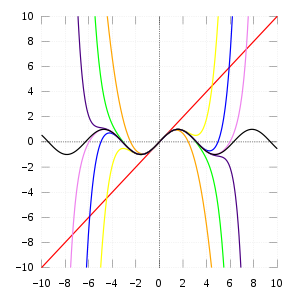
\includegraphics[scale=0.7]{taylor_series}

In Calculus I we covered linear approximation. We would find a linear function tangent to a function at a point $ a $, and for values very close to $ a $ our linear function would approximate the target function. Taylor series are the same thing, except we're raising our linear approximation to a higher degree. This increases the "neighborhood" of values around $ a $, increasing the accuracy of the approximation and allowing us to approximate values further away from $ a $. If we built a Taylor polynomial with $ \infty $ terms, it would exactly match the original function. You can see this in the image above; each new function is more closely modeling $ sin(x) $.

%\subsection{Taylor Series Remainders}
%Given a function $ f(x) $ and it's Taylor polynomial $ T(x) $ centered at $ a $, for any degree of the Taylor polynomial, $ f(a) = T(a) $. Take a look at the expanded definition of a Taylor series. Plugging in $ x = a $ will elimate all terms with $ (x - a) $ in them. This leaves only the first term, $ f(a) $:
%
%$$ T(x) = f(a) + \frac{f'(a)}{1!}(x-a) + \frac{f''(a)}{2!}(x-a)^2 + \cdots $$
%$$ T(a) = f(a) $$
%
%\noindent This is also graphically evident by looking at the graph of the function and the Taylor polynomial. At $ x = a $, they will meet. See the image above.
%
%So for 


%$$ R_n(x) = \frac{f^{(n+1)}(c)}{(n+1)!}(x-a)^{n+1} $$



\subsection*{Examples}
\begin{enumerate}
	\item Find the first 4 nonzero terms ofthe Taylor polynomial for the function $ f(x) = sin(x) $ centered at $ a = 0 $ \\
	
	\textbf{Step 1.} Expanding the definition of Taylor series above to 4 terms, we get
	$$
		f(a) + f'(a)(x-a) + \frac{f''(x)}{2!}(x-a)^2 + \frac{f'''(x)}{3!}(x-a)^3
	$$
	\textbf{Step 2.} We can see that we're going to need up to the 3rd derivative of $ f(x) $, so I'm going to write all those out here
	$$ f(x) \quad\quad f'(x) \quad\quad f''(x) \quad\quad f'''(x)$$
	$$ sin(x) \to cos(x) \to -sin(x) \to -cos(x) $$
	\textbf{Step 3.} Now we can substitute the derivatives we just found, and $ a = 0 $, to find our 3rd degree Taylor polynomial
	
	$$ sin(0) + cos(0)\cdot x - \frac{sin(0)}{2!}x^2 - \frac{cos(0)}{3!}x^3 $$

	We can simplify and elimate some terms. For this specific series, you can see that every other term (1st, 3rd, etc...) contains $ sin(0) = 0 $ which will elimate every other term. This is because $ a = 0 $. We can also simplify $ cos(0) = 1 $.
	$$ x - \frac{x^3}{3!} $$
	Our task was to find the first 4 nonzero terms. We found 4 terms, but 2 of them were zero. Usually we would go back to step 2 and add more terms, but for this Taylor polynomial it is easy to see the pattern:
	$$ x - \frac{x^3}{3!} + \frac{x^5}{5!} - \frac{x^7}{7!} $$
	
	
	
	\item Find the first four nonzero terms of the Taylor series for the function $ f(x) $ centered at $ a $, then write a power series using summation notation\\
	$$ f(x) = \frac{4}{x} \quad \quad \quad a = 1 $$
	
	We can skip writing out the expanded definition, we'll just use the shorter summation definition. Let's just write the derivatives of this function for now:
	$$ f(x) \quad f'(x) \quad f''(x) \quad f'''(x) $$
	$$ \frac{4}{x} \to -\frac{4}{x^2} \to \frac{8}{x^3} \to -\frac{24}{x^4} $$

	Now we can fill in the definition with our found derivatives, and $ a = 1 $
	$$ \sum_{n=0}^{\infty} \frac{f^{(n)}(a)}{n!}(x-a)^n $$
	$$ f(1) + f'(1)(x-1) + \frac{f''(1)(x-1)^2}{2!} + \frac{f'''(1)(x-1)^3}{3!} $$
	$$ 4 - 4(x-1) + 4(x-1)^2 - 4(x-1)^3 $$


\end{enumerate}	



\pagebreak


\section{Series Strategies}

\begin{itemize}
	
	\item[] For factorial, exponential, and some polynomial functions, use the \textbf{Ratio Test}.

	\item[] For series of the form $ \sum \left( \sim \right)^n $, use the \textbf{Root Test}.

	\item[] For series of the form $ \sum \frac{\text{polynomial}}{\text{polynomial}} $ use the \textbf{Limit Comparison Test} or the \textbf{P-series Test}.

	\item[] For inequalities like $ \left| \sin(\sim) \right| \leq \sum \sim $, use the \textbf{Direct Comparison Test}

	\item[] For series of the form $ \sum \frac{\ln(\sim)}{\text{polynomial}} $, then sometimes use the \textbf{Integral Test}.
	
	\item[] If there's an alternating bit like $ (-1)^n $ or $ (-1)^{n+1} $, use the \textbf{Alternating Series Test}.
\end{itemize}


\pagebreak


\chapter{Tables}

\section{Table of Derivatives}
\begin{center}
\begin{large}

\textbf{Polynomials}
\def\arraystretch{1.5}
\begin{tabular}{ c | c | c }
	$ \frac{d}{dx} \; c = 0 $ &
	$ \frac{d}{dx} \; x = 1 $ &
	$ \frac{d}{dx} \; x^n = nx^{(n-1)} $ \\
\end{tabular}

\bigskip
\bigskip

\textbf{Exp/Log}
\begin{tabular}{ c | c | c }
	$ \frac{d}{dx} \; e^x = e^x $ &
	$ \frac{d}{dx} \; a^x = a^x \ln(a) $ &
	$ \frac{d}{dx} \; \ln(x) = \frac{1}{x} $ \\
\end{tabular}

\bigskip
\bigskip

\textbf{Trigonometric}
\bigskip
\def\arraystretch{1.5}
\begin{tabular}{ c | c }
	$ \frac{d}{dx} \; sin(x) = cos(x) $ &
	$ \frac{d}{dx} \; csc(x) = -csc(x)cot(x) $ \\

	\hline	
	
	$ \frac{d}{dx} \; cos(x) = -sin(x) $ &
	$ \frac{d}{dx} \; sec(x) = sec(x)tan(x) $ \\
	
	\hline
	
	$ \frac{d}{dx} \; tan(x) = sec^2(x) $ &
	$ \frac{d}{dx} \; cot(x) = -csc^2x $ \\
	

\end{tabular}

\bigskip
\bigskip

\textbf{Inverse Trigonometric}
\bigskip
\def\arraystretch{1.5}
\begin{tabular}{ c | c  }
	$ \frac{d}{dx} \; arcsin(x) = \frac{1}{\sqrt{1-x^2}} $ &
	$ \frac{d}{dx} \; arccsc(x) = \frac{-1}{|x|\sqrt{x^2-1}} $ \\

	\hline	
	
	$ \frac{d}{dx} \; arccos(x) = \frac{-1}{\sqrt{1-x^2}} $ &
	$ \frac{d}{dx} \; arcsec(x) = \frac{1}{|x|\sqrt{x^2-1}} $ \\
	
	\hline
	
	$ \frac{d}{dx} \; arctan(x) = \frac{1}{1+x^2} $ &
	$ \frac{d}{dx} \; arccot(x) = \frac{-1}{1+x^2} $ \\
	

\end{tabular}

\end{large}
\end{center}




\section{Table of Integrals}
\begin{center}
\begin{large}

\textbf{Basic Forms}

\bigskip
\def\arraystretch{1.5}
\begin{tabular}{ c | c }
	$ \int x^n \; dx = \frac{1}{n+1}x^{n+1}  \quad \quad $ &
	$ \quad \quad \int \frac{1}{x} \; dx = \ln|x| $ \\
	
	\hline

	$ \int ud \; dv = uv - \int v \; du  \quad \quad $ &
	$ \quad \quad \int e^x \; dx = e^x $ \\
\end{tabular}



\end{large}
\end{center}




\end{document}
